\documentclass[a4paper, 12pt]{article}
\usepackage[top=2cm, bottom=2cm, left=2.5cm, right=2.5cm]{geometry}

\usepackage[utf8]{inputenc}
\usepackage[brazilian]{babel}
\usepackage{indentfirst}

\usepackage{graphicx}
\usepackage[pdftex]{hyperref}
\graphicspath{ {imagens/} }
\usepackage{xcolor}

%Caracteres Japoneses
\usepackage{CJK}

% Definindo novas cores
\definecolor{verde}{rgb}{0.25,0.5,0.35}
\definecolor{jpurple}{rgb}{0.5,0,0.35}



\begin{document}
\begin{titlepage} %iniciando a "capa"
	\begin{center} %centralizar o texto abaixo
		{\large Unicamp}\\[0.2cm] %0,2cm é a distância entre o texto dessa linha e o texto da próxima
		{\large LA111}\\[0.2cm] % o comando \\ "manda" o texto ir para próxima linha
		{\large Prof. Bartira Takiuti Ginde}\\[3.2cm]
		{\bf \huge Japonês I}\\[5.1cm] % o comando \bf deixa o texto entre chaves em negrito. O comando \huge deixa o texto enorme
	\end{center} %término do comando centralizar
	{\large Erik Yuji Goto}\\[0.5cm] % o comando \large deixa o texto grande
	{\large RA: 234009}\\[10cm]
	\begin{center}
		{\large Campinas}\\[0.2cm]
		{\large 2020}
	\end{center}
\end{titlepage} %término da "capa"

\tableofcontents

\newpage
\section{Horas}
	\Large
	\textbf{Horas}
	\normalsize
	\begin{CJK}{UTF8}{min}
		\begin{enumerate}
			\item いちじ
			\item にじ
			\item さんじ
			\item よじ *
			\item ごじ
			\item ろくじ
			\item しちじ *
			\item はちじ
 			\item くじ
			\item じゅうじ
			\item じゅういちじ
			\item じゅうにじ
		\end{enumerate}
	\textbf{ごぜん} - AM\\
	\textbf{ごご} - PM
	
	\Large
	\textbf{Minutos}\\
	\normalsize
	5 - ごふん\\
	10 - じゅつぷん  \\
	
	\Large
	\textbf{Pergunta}\\
	\normalsize
	いま\textbf{なん}じです\textbf{か}。\\
	さんぱうろはいま\textbf{なん}じです\textbf{か}。
	\end{CJK}

\newpage
\section{Autoapresentacao}
	\begin{CJK}{UTF8}{min}
		Meu nome e: わたじのなまえは...です\\
		... e meu amigo: ...はわたしのともだちです\\
		... e minha universidade: ...はわたじのだいがくです\\
		Eu sou estudante de japones: わたじはにほんごのがくせいです\\
		Meu curso e: わたじのせんこうは...です\\
		
		*Universidade Estadual de Campinas: カンピ-ナスじゅうりつだいがく\\
		
		\Large
		\textbf{Ano Escolar}\\
		\normalsize
			\begin{enumerate}
				\item いちねんせい
				\item にねんせい
				\item さんえんせい
				\item よねんせい
				\item ごねんせい
			\end{enumerate}
		
		\Large
		\textbf{Idade}\\
		\normalsize
		\begin{figure}[h]
			\centering
			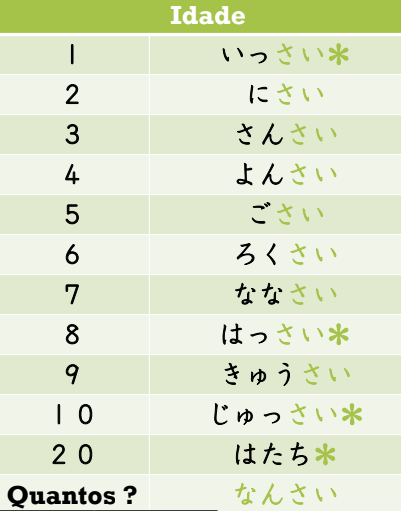
\includegraphics[width=0.5\linewidth]{Imagens/idade}
			\caption{Idade}
			\label{fig:idade}
		\end{figure}
		
		
		
		
	\end{CJK}

\newpage
\section{Numeros}
	\begin{CJK}{UTF8}{min}
		\Large
		\textbf{ひゃく}
		\normalsize
	
\begin{figure}[h]
	\centering
	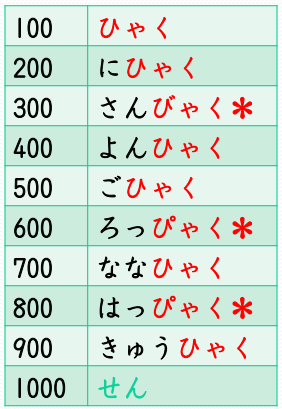
\includegraphics[width=0.3\linewidth]{Imagens/hyaku}
	\caption{ひゃく}
	\label{fig:hyaku}
\end{figure}

	\Large
	\textbf{せん}
	\normalsize
	\begin{figure}[h]
		\centering
		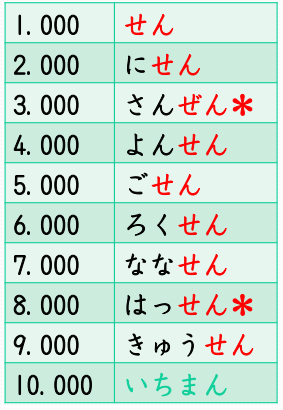
\includegraphics[width=0.3\linewidth]{Imagens/sen}
		\caption{せん}
		\label{fig:sen}
	\end{figure}
	\newpage
	\Large
	\textbf{まん}
	\normalsize
	\begin{figure}[h]
		\centering
		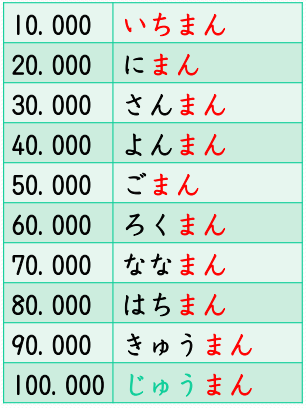
\includegraphics[width=0.3\linewidth]{Imagens/man}
		\caption{まん}
		\label{fig:man}
	\end{figure}
	
	
	\end{CJK}

	
	\begin{CJK}{UTF8}{min}
		\Large
		\textbf{Quanto Custa?}\\
		\normalsize
		[...]はいくらですか
	\end{CJK}




\newpage
\section{Pronome Demonstrativo}
\subsection{kore, sore, are, dare (Aula 9)}
\begin{CJK}{UTF8}{min}

	\begin{itemize}
		\item これ - Isto(quando se refere a um objeto que esta \textit{perto} da pessoa)\\
		\item それ - Isso(quando se refere a um objeto que esta \textit{longe} da pessoa)\\
		\item あれ - Aquilo(quando se refere a um objeto que esta longe das duas pessoas)\\
		
		\item \textbf{どれ} - Qual?
		
	\end{itemize}
	
	\textbf{Exemplos:}\\
	これ\textbf{は}___です。\\
	それ\textbf{は}___です \\
	あれ\textbf{は}___です。\\
	
	\textbf{Perguntas:}\\
	これはなんです\textbf{か}\\
	
	
	
	\textbf{Objeto pertencente a alguem:}\\
	これは___の___です。\\(PESSOA) +(OBJETO \\
	
	\textbf{Este objeto pertence a quem:?}\\
	これは\textbf{だれ}のほんですか。
\end{CJK}

\subsection{kono, sono, ano (Aula 10)}
\begin{CJK}{UTF8}{min}
	\begin{itemize}
		\item この - Este(quando se refere a um objeto que esta \textit{perto} da pessoa)\\
		\item その - Esse(quando se refere a um objeto que esta \textit{longe} da pessoa)\\
		\item あの - Aquele(quando se refere a um objeto que esta longe das duas pessoas)\\
	\end{itemize}

	\textbf{Exemplo:}\\
	Esta e a caneta da Ayako sensei.\\
	このペンはあやこせんせいのです。	\\
	
	\textbf{Ao pedir algo(em contexto de compra):}\\
	をください\\
	コーラ\textbf{をください}。\\
	しんぶん\textbf{をください}。\\
	\textbf{この}Tシャツ\textbf{をください}。\\
	
\end{CJK}
	
\section{koko, soko, asoko (Aula 11)}	
\begin{CJK}{UTF8}{min}
	\begin{itemize}
		\item ここ - Aqui\\
		\item そこ - Ai\\
		\item あそこ - La/Ali\\
	\end{itemize}

	\textbf{Exemplos:}\\
	ここはゆうびんきょくです。(Aqui e o correio)\\
	田中さんはあそこです。 (O senhor Tanaka esta ali)\\
\end{CJK}

\section{Mo/tambem (Aula 12)}
\begin{CJK}{UTF8}{min}
	これ\textbf{は}1800円です。$ -> $ これ\textbf{も}1800円です。\\
	
	あのようこさ\textbf{は}にほんじんです。$ -> $ みやざきさん\textbf{も}(にほんじん)です。\\
	
	\textbf{Presente Afirmativo:}\\
	です\\
	
	\textbf{Presente Negativo:}\\
	ではありませなん\\
	
	
\end{CJK}

\section{Ne, Yo (Aula 13)}
\begin{CJK}{UTF8}{min}
	ね e usado quando o falante esta buscando a confirmaçao / acordo do ouvinte de acordo com	o que foi dito. Pode ser traduzido como:\\
	“certo?”, “ne?”.\\
	これはとんかつです\textbf{ね}。\\
	
	よ é usado quando o falante tem certeza do que está falando e está passando uma	informação nova ao ouvinte. Pode ser traduzido como: \\
	“viu”, “eu te digo”.\\
	これはとんかつです\textbf{よ}。\\
	
	と é uma partícula aditiva. É usada para somar	os objetos ou pratos que você deseja pedir.	Pode ser traduzido como: \\“e”.\\
	ラーメン\textbf{と}とんかつをください。\\
	
	
\end{CJK}

\section{Verbos de Acao (Aula 15)}
	\begin{CJK}{UTF8}{min}
		\Large
		おきまる(Grupo II):Acordar\\
		\normalsize
		おき\textcolor{red}{ます}\\
		おき\textcolor{red}{ません}\\
		おき\textcolor{red}{ました}\\
		おき\textcolor{red}{ませんでした}\\

		\Large
		ねる(Grupo II):Dormir\\
		\normalsize
		ね\textcolor{red}{ます}\\
		ね\textcolor{red}{ません}\\
		ね\textcolor{red}{ました}\\
		ね\textcolor{red}{ませんでした}\\
		
		\Large
		いく(Grupo I):Ir\\
		\normalsize
		い\textcolor{green}{き}\textcolor{red}{ます}\\
		い\textcolor{green}{き}\textcolor{red}{ません}\\
		い\textcolor{green}{き}\textcolor{red}{ました}\\
		い\textcolor{green}{き}\textcolor{red}{ませんでした}\\
		
		\Large
		かえる(Grupo I):Voltar\\
		\normalsize
		かえ\textcolor{green}{り}\textcolor{red}{ます}\\
		かえ\textcolor{green}{り}\textcolor{red}{ません}\\
		かえ\textcolor{green}{り}\textcolor{red}{ました}\\
		かえ\textcolor{green}{り}\textcolor{red}{ませんでした}\\
		
		\Large
		くる(Grupo III):Dormir\\
		\normalsize
		き\textcolor{red}{ます}\\
		き\textcolor{red}{ません}\\
		き\textcolor{red}{ました}\\
		き\textcolor{red}{ませんでした}\\
		
		\Large
		Exemplos:\normalsize
		\begin{itemize}
			\item \colorbox{green}{すずきさんは}\colorbox{yellow}{きょう}\colorbox{orange}{ぎんごうに}\colorbox{blue}{いきました}\\
			\colorbox{green}{Sujeito \textcolor{red}{は}}\colorbox{yellow}{tempo}\colorbox{orange}{lugar \textcolor{red}{に}}\colorbox{blue}{Verbo de deslocamento}\\
			O Sr. Suzuki foi para o banco hoje
			
			\item \colorbox{green}{とよたさんは}\colorbox{yellow}{あしたくじに}\colorbox{orange}{だいがくに}\colorbox{blue}{きます}\\
			\colorbox{green}{Sujeito \textcolor{red}{は}}\colorbox{yellow}{tempo + tempo に}\colorbox{orange}{lugar \textcolor{red}{に}}\colorbox{blue}{Verbo de deslocamento}\\
			O Sr.Toyota vem para a faculdade às 9 horas amanha
			
			\item \colorbox{green}{くろださんは}\colorbox{yellow}{きのう}\colorbox{gray}{ひとりで}\colorbox{orange}{えいがに}\colorbox{blue}{いきました}\\
			\colorbox{green}{Sujeito \textcolor{red}{は}}\colorbox{yellow}{tempo + tempo に}\colorbox{gray}{companhia \textcolor{red}{と}}\colorbox{orange}{lugar \textcolor{red}{に}}\colorbox{blue}{Verbo de deslocamento}\\
			Sr. Kuroda foi para o cinema sozinho ontem

		\end{itemize}
		
		\begin{figure}[h]
			\centering
			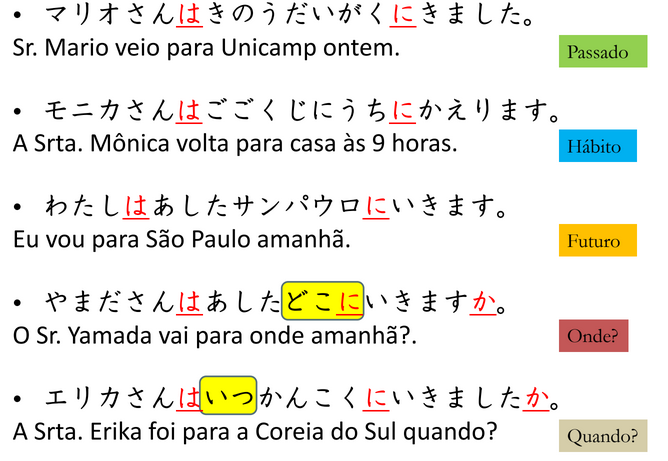
\includegraphics[width=0.7\linewidth]{Imagens/ex1}
			\caption{Mais Exemplos}
			\label{fig:ex1}
		\end{figure}
	\newpage
	\Large
	Tempo relativo\\
	\normalsize	
	\begin{figure}[h]
		\centering
		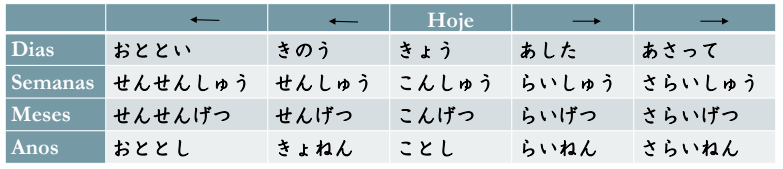
\includegraphics[width=1\linewidth]{Imagens/tempo_relativo}
		\caption{Tempo Relativo}
		\label{fig:temporelativo}
	\end{figure}
		
	\Large
	Formula Geral\\
	\normalsize
	
	\colorbox{green}{Sujeito \textcolor{red}{は}}\colorbox{yellow}{tempo + tempo \textcolor{red}{に}}\colorbox{gray}{complemento \textcolor{red}{と}}\colorbox{cyan}{M. transporte \textcolor{red}{て}}\colorbox{orange}{lugar \textcolor{red}{に}}\colorbox{blue}{V. deslocamento}\\

		
	\end{CJK}

\newpage
\section{Verbos de Acao}
	\begin{CJK}{UTF8}{min}
		\Large
		Grupos de Verbos\\
		\normalsize
		\begin{figure}[h]
			\centering
			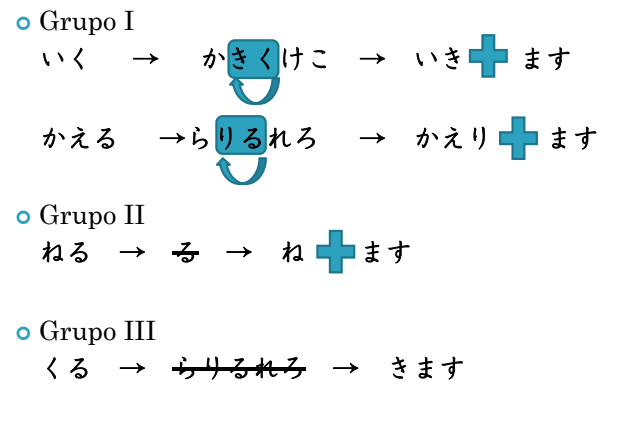
\includegraphics[width=0.8\linewidth]{Imagens/grupos_verbos}
			\caption{Grupos de Verbos}
			\label{fig:gruposverbos}
		\end{figure}
	
		\Large
		Formula \\
		\normalsize
		\colorbox{green}{Sujeito \textcolor{red}{は}}\colorbox{yellow}{Temp \textcolor{red}{に}}\colorbox{pink}{Compl \textcolor{red}{と}}\colorbox{cyan}{Lugar \textcolor{red}{で}}\colorbox{red}{Obj. Direto \textcolor{white}{は}}\colorbox{cyan}{V. acao}
		\begin{figure}[h]
			\centering
			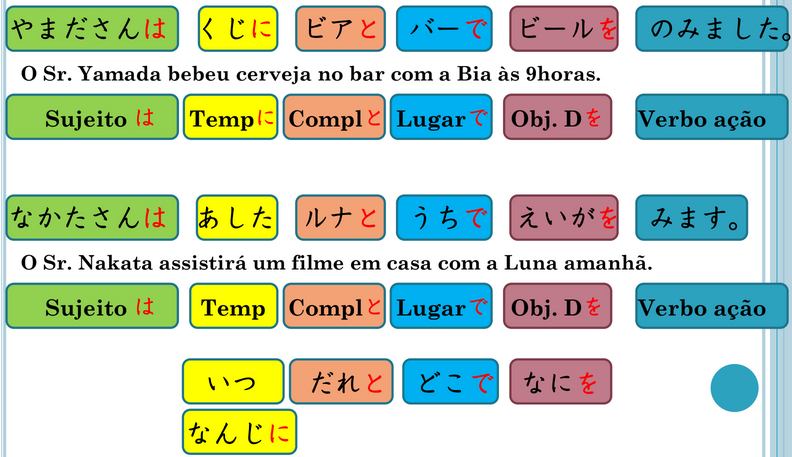
\includegraphics[width=0.8\linewidth]{Imagens/vacao}
			\caption{Exemplos}
			\label{fig:vacao}
		\end{figure}
		
		\newpage
		\Large
		\textcolor{red}{Obs: Tempo}
		\normalsize
			\begin{figure}[h]
				\centering
				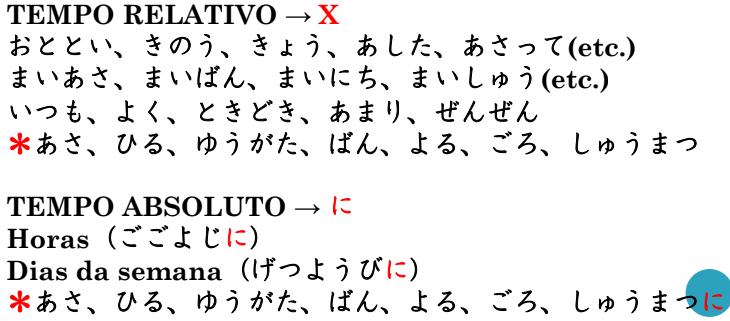
\includegraphics[width=0.85\linewidth]{Imagens/tempo}
				\caption{Particula に}
				\label{fig:tempo}
			\end{figure}
		
		\Large
		\textbf{Convite}\\
		\normalsize
		ゆいさん、きょうともだちかくしょくにいき\textcolor{red}{ませんか}\\
		(Yui, voce nao quer/nao gostaria de ir para o bandejao com
		amigos hoje?) - Convidando
		
		ええ、いいですね/はい、いいですね\\
		Sim, que bom!\\
		すみませんが、ちょ\underline{つ}と...\\
		Desculpe mas...\\
		うーん、きょうはちょ\underline{つ}と...\\
		Hum...Hoje...
	\end{CJK}
\newpage



\section{Verbos de Existencia}
\begin{CJK}{UTF8}{min}
	Classificacao:
	\begin{itemize}
		\item Seres Inanimados - ある
		\item Seres Animados - いる
	\end{itemize}
\end{CJK}
\subsection{Estrutura}
	\begin{CJK}{UTF8}{min}
		Lugar \textcolor{red}{に} + ser \textcolor{red}{が} + verbo de existência.\\
		つくえの上\textcolor{red}{に}本\textcolor{red}{が}あります。\\
		\textbf{Pergunta:}\\
		つくえの上に\textcolor{red}{なにが}あります\textcolor{red}{か}。\\
		"Nao tem nada"\\
		つくえの上に\textcolor{red}{なにも}ありません。\\
		
	\end{CJK}
\subsection{Evento}
	\begin{CJK}{UTF8}{min}
		Tempo\textcolor{red}{に} + Lugar\textcolor{red}{で} + Evento\textcolor{red}{が} + あります。\\
		しゅまつ\textcolor{red}{に}サンパウロ\textcolor{red}{で}パーテイー\textcolor{red}{が}あります。
	\end{CJK}

\subsection{Foco no ser}
\begin{CJK}{UTF8}{min}
	Ser\textcolor{red}{は} + Local\textcolor{red}{に} + あります/います。\\
	山田さんはこうえんにいます。 
\end{CJK}

\section{Particula mo}

\begin{CJK}{UTF8}{min}
	Nas particulas \textcolor{red}{は、が、を} tira a particula e acrescenta \textcolor{red}{も}.
\end{CJK}

\section{Adjetivos}
\begin{CJK}{UTF8}{min}
	\begin{table}[h]
		\caption{Adjetivo に}
		\begin{tabular}{lllll}
			& Afirmativo & Negativo &   \\
			Presente & たか\textbf{い}です          & たか\textbf{くない}です         \\
			Passado  & たか\textbf{かっかた}です          & たか\textbf{くなっかた}です         \\

		\end{tabular}
	\end{table}
	\textbf{Excecao:} いいです e かっこいい\\いいですーよくないですーよかったですーよくなかったです
	
	\begin{table}[h]
		\caption{Adjetivo な}
		\begin{tabular}{lllll}
			& Afirmativo & Negativo &   \\
			Presente & ひま\textbf{です}          & ひま\textbf{ではありません}         \\
			Passado  & ひま\textbf{でした}          & ひま\textbf{ではありませんでした}         \\
			
		\end{tabular}
	\end{table}
\end{CJK}

\subsection{Perguntando}
\begin{CJK}{UTF8}{min}	
	\textcolor{red}{どう}(como) - Perguntar sobre a impressao ou opiniao a cerca de alguma coisa.\\
	\textcolor{red}{どんな}(que tipo) - Para perguntar sobre a descricao de algo.\\
	\textcolor{red}{だれ}(qual) - Solicitar que o ouvinte escolha uma entre as mais de duas alternativas.
\end{CJK}

\section{Gostar/Odiar}
\begin{CJK}{UTF8}{min}
	にく\textcolor{red}{が}すきです\\
	えいあを\textbf{見る}\textcolor{red}{の}\textcolor{blue}{が}すきです\\
	
	\textbf{(Intensificando)}\\
	えいがを見るのが\textcolor{red}{ほんとうに}すきです\\
	
	\textbf{Respondendo "tanto faz"}\\
	すきでもきらいでもありません\\
	
	\textbf{Evite usar きらいです, uma forma mais educada é usar:}\\
	あまりすきではありません\\
	
	\textbf{Eu \textcolor{green}{gostei} de praia}\\
	私はうみが\textcolor{red}{きにいりました}
	
	\subsection{Perguntas}
		\begin{enumerate}
			\item どんなスポーツすきですか
			\item どんなおんがくすきですか
			\item どんなえいがすきですか
		\end{enumerate}
\end{CJK}

\section{Objeto Indireto}
\begin{CJK}{UTF8}{min}
	Sujeito\textcolor{red}{は} + Tempo\textcolor{red}{に} + Lugar\textcolor{red}{で} + Obj.Indireto\textcolor{blue}{に} + Obj.Direto\textcolor{red}{を} + Verbo
\end{CJK}

\section{Convites}
\begin{CJK}{UTF8}{min}
	今日ともだちとがくしょくにいき\textbf{ましょう}\\
	今日ともだちとがくしょくにいき\textbf{ましょうか}\\
	
	ええ、いきましょう
	すみませんが、ちょっと。。。
\end{CJK}





\newpage
\section{Vocabulario}
\subsection{Contagem}
\subsubsection{Pessoas}
\begin{CJK}{UTF8}{min}
	\begin{enumerate}
		\item ひとり
		\item ふたり
		\item さにん
		\item よにん\\...
	\end{enumerate}	
\end{CJK}

\subsubsection{Objetos Achatados}
\begin{CJK}{UTF8}{min}
	\begin{enumerate}
		\item いちまい
		\item にまい
		\item さにまい
		\item よんまい\\...
	\end{enumerate}	
\end{CJK}

\subsubsection{Carros, maquinas, etc}
\begin{CJK}{UTF8}{min}
	\begin{enumerate}
		\item いちだい
		\item にだい
		\item さにだい
		\item よんだい\\...
	\end{enumerate}	
\end{CJK}

\subsubsection{Quilograma}
\begin{CJK}{UTF8}{min}
	\begin{enumerate}
		\item いちキロ
		\item にキロ
		\item さにキロ
		\item よんキロ\\...
	\end{enumerate}	
\end{CJK}

\subsubsection{Objetos finos e achatados}
\begin{CJK}{UTF8}{min}
	\begin{enumerate}
		\item いっぽん
		\item にほん
		\item さんぼん
		\item よんほん
		\item ごほん
		\item ろっぽん
		\item ななんほん
		\item はっぽん
		\item きゅほん
		\item じゅっぽん
		\item じゅういっぽん\\...
	\end{enumerate}	
\end{CJK}

\subsubsection{Uso Generico}
\begin{CJK}{UTF8}{min}
	\begin{enumerate}
		\item ひとつ
		\item ふたつ
		\item みっつ
		\item よっつ
		\item いつつ
		\item むっつ
		\item ななつ
		\item やっつ
		\item ここのつ
		\item とお
		\item じゅういち\\...
	\end{enumerate}	
\end{CJK}
\subsection{Mes}
	\begin{CJK}{UTF8}{min}
		\begin{itemize}
			\item いちがつ (一月)\\...
			\item しがつ (四月)\\...
			\item しちがつ (七月)\\...
			\item くがつ (九月)\\...
		\end{itemize}
		
	\end{CJK}

\subsection{Adjetivos}
\begin{CJK}{UTF8}{min}
	\begin{itemize}
		\item おおきい
		\item ちいさい\\
		
		\item たかい
		\item やすい\\
		
		\item あたらしい
		\item ふるい\\
		
		\item あっつい
		\item さむい
		\item つめたい\\
		
		\item おもしろい
		\item つまらない\\
		
		\item おいしい
		\item まずい\\
		
		\item いい
		\item わるい\\
		
		\item たのしい\\
		
		\item こわい\\
		
		\item はやい
		\item おそい\\
		
		\item むずかしい
		\item やさしい\\
		
		\item きれい(な)
		\item きたない\\
		
		\item かっこいい
		\item ハンサム(な)\\
		
		\item いそがしい
		\item ひま(な)\\
		
		\item しずか
		\item にぎやか(な)\\
		
		\item 元気
	\end{itemize}
	
\subsection{Adverbio de Intensidade}
	\begin{itemize}
		\item おんとうに
		\item すごく
		\item とても
		\item すこし
		\item ちょっと
		\item あまり
		\item ぜんぜん
	\end{itemize}
\end{CJK}




































































\newpage
%Japones 1
\begin{CJK}{UTF8}{min}
	\paragraph{Verbos}
	\begin{itemize}
		\item おきる:Acordar \textbf{(Grupo II)}
		\item ねる:Dormir \textbf{(Grupo II)}
		\item いく:Ir \textbf{Grupo I}
		\item かえる:Voltar(para casa) \textbf{(Grupo I)}
		\item くる:Vir \textbf{(Grupo III - きます)}
		\item たべる:Comer \textbf{(Grupo II)}
		\item のむ:Beber \textbf{(Grupo I)}
		\item きく:Ouvir \textbf{(Grupo I)}
		\item よむ:Ler \textbf{Grupo I)}
		\item はなす:Falar \textbf{(Grupo I)}
		\item みる:Assistir \textbf{(Grupo II)}
		\item テニスする:Jogar tenis \textbf{(Grupo III)}
		\item べんきょうする:Estudar \textbf{(Grupo III)}
	\end{itemize}
\paragraph{Lugares}
	\begin{itemize}
		\item き\underline{つ}さてん/カフ\underline{エ}¥: Cafeteria
		\item ぎんこう: Banco
		\item トイレ: Banheiro
		\item としょかん: Biblioteca
		\item ゆうびんきょく: Correio
		\item がくしょく: Bandejão
		\item えいが:Cinema
		\item バー:Bar
		\item いえ/うち:Casa(Lar)
	\end{itemize}

\paragraph{Meios de Transporte}
	\begin{itemize}
		\item てんし\underline{や}:Trem
		\item ちかてつ:Metro
		\item くるま:Carro
		\item タクシー:Taxi
		\item しんかんせん:Trem Bala
		\item ひこうき:Aviao
		\item バス:Onibus
		\item じてんじ\underline{ゃ}:Bicicleta
		\item バイク:Moto
		\item ふね:Navio
	\end{itemize}

\paragraph{Diversos}
	\begin{itemize}
		\item あさ:Manha
		\item ひる:Tarde
		\item ゆうがた:Crespusculo
		\item ばん/よる:Noite/Madrugada
		\item あさごはん:Cafe da Manha
		\item ひるごはん:Almoco
		\item ばんごはん:Janta
		\item テレビ:TV
		\item えいが:Cinema/Filme
		\item ざ\underline{つ}し:Revista
		\item おんがく:Musica
		\item スポーツ:Esporte
		\item デート:Encontro Romantico(date)
	\end{itemize}

\paragraph{Comidas/Bebidas}
	\begin{itemize}
		\item さかな:Peixe
		\item とんかつ:Tonkatsu
		\item にく:Carne
		\item やさい:Vegetais
		\item おいしい:Gostoso!
		\item まずい:Ruim :c
		\item コーヒー:Cafe
		\item ジ\underline{ュ}ース:Suco
		\item みず:Agua
		\item ミルク/ぎ\underline{ゅ}うにゆう:Leite
		\item おち\underline{ゃ}:Cha
		\item おさけ:Bebida Alcoolica
		\item ハンバーガー:Hamburguer
		\item アイスクリーム:Sorvete
\end{itemize}

\paragraph{Objetos}
	\begin{itemize}
		\item えんぴつ:Lapis
		\item メニュー:Menu(de restaurante)
		\item かさ:Guarda Chuva
		\item かばん:Bolsa
		\item くつ:Sapato
		\item さいふ:Carteira
		\item ジーンズ:Jeans
		\item じしょ:Dicionario
		\item じてんし\textit{や}:Bicicleta
		\item しんぶん:Jornal
		\item Tシ\textit{ヤ}ツ:Camiseta
		\item とけい:Relogio
		\item ノート:Caderno
		\item ぼうし:Chapeu
		\item ほん:Livro
		\item コンピューター:Computador	
		

	\end{itemize}
\end{CJK}

\paragraph{Dias da Semana}
		\begin{CJK}{UTF8}{min}
			\begin{itemize}
				\item げつようび:Segunda
				\item かようび:Terca
				\item すいようび:Quarta
				\item もくようび:Quinta
				\item きんょうび:Sexta
				\item どようび:Sabado
				\item にちようび:Domingo
				\item しゅうまつ:Fm de semana
				
			\end{itemize}
		\end{CJK}

\paragraph{Todo[...]}
	\begin{CJK}{UTF8}{min}
		\begin{itemize}
			\item まいあさ/まいばん:Toda manha/Toda Noite
			\item まいにち:Todo dia
			\item まいし\textit{ゅ}う:Toda semana
			\item まいつき:Todo mês
			\item まいとし:Todo ano
			\item まいげつようび:Toda segunda-feira
		\end{itemize}
	\end{CJK}

\paragraph{Frequencia}
	\begin{CJK}{UTF8}{min}
		\begin{itemize}
			\item いつも:Sempre
			\item よく:Frequentemente
			\item たいてい:Geralmente
			\item ときどき:As vezes
			\item あまり:Nao muito $ \star $
			\item ぜんぜん:Quase nunca $ \star $
		\end{itemize}
	$ \star $ verbo negativo
	\end{CJK}


\end{document}